\documentclass{article}\usepackage[]{graphicx}\usepackage[]{color}
%% maxwidth is the original width if it is less than linewidth
%% otherwise use linewidth (to make sure the graphics do not exceed the margin)
\makeatletter
\def\maxwidth{ %
  \ifdim\Gin@nat@width>\linewidth
    \linewidth
  \else
    \Gin@nat@width
  \fi
}
\makeatother

\definecolor{fgcolor}{rgb}{0.345, 0.345, 0.345}
\newcommand{\hlnum}[1]{\textcolor[rgb]{0.686,0.059,0.569}{#1}}%
\newcommand{\hlstr}[1]{\textcolor[rgb]{0.192,0.494,0.8}{#1}}%
\newcommand{\hlcom}[1]{\textcolor[rgb]{0.678,0.584,0.686}{\textit{#1}}}%
\newcommand{\hlopt}[1]{\textcolor[rgb]{0,0,0}{#1}}%
\newcommand{\hlstd}[1]{\textcolor[rgb]{0.345,0.345,0.345}{#1}}%
\newcommand{\hlkwa}[1]{\textcolor[rgb]{0.161,0.373,0.58}{\textbf{#1}}}%
\newcommand{\hlkwb}[1]{\textcolor[rgb]{0.69,0.353,0.396}{#1}}%
\newcommand{\hlkwc}[1]{\textcolor[rgb]{0.333,0.667,0.333}{#1}}%
\newcommand{\hlkwd}[1]{\textcolor[rgb]{0.737,0.353,0.396}{\textbf{#1}}}%

\usepackage{framed}
\makeatletter
\newenvironment{kframe}{%
 \def\at@end@of@kframe{}%
 \ifinner\ifhmode%
  \def\at@end@of@kframe{\end{minipage}}%
  \begin{minipage}{\columnwidth}%
 \fi\fi%
 \def\FrameCommand##1{\hskip\@totalleftmargin \hskip-\fboxsep
 \colorbox{shadecolor}{##1}\hskip-\fboxsep
     % There is no \\@totalrightmargin, so:
     \hskip-\linewidth \hskip-\@totalleftmargin \hskip\columnwidth}%
 \MakeFramed {\advance\hsize-\width
   \@totalleftmargin\z@ \linewidth\hsize
   \@setminipage}}%
 {\par\unskip\endMakeFramed%
 \at@end@of@kframe}
\makeatother

\definecolor{shadecolor}{rgb}{.97, .97, .97}
\definecolor{messagecolor}{rgb}{0, 0, 0}
\definecolor{warningcolor}{rgb}{1, 0, 1}
\definecolor{errorcolor}{rgb}{1, 0, 0}
\newenvironment{knitrout}{}{} % an empty environment to be redefined in TeX

\usepackage{alltt}
\IfFileExists{upquote.sty}{\usepackage{upquote}}{}
\begin{document}

\title {\textbf{United States School Statistics: Chicago, Illinois}
\\ IT497 OSEMN Assignment}
\author { Sonali Changkakoti
\\ School of Information Technology 
\\ Illinois State University
\\
\texttt{schangk@ilstu.edu}}
\date{\today} 
\maketitle


\section{Introduction}
Schools in the United States comprise of both public as well as private schools. The funding and control of public schools are done by state, local and federal government. Their curricula and staffing are decided by the locally elected school boards. On the other hand, private schools are generally free to determine their own curricula and staffing policies. There are also charter schools, which receive public funding but operate independently. Some states do not have charter school authorization. Around 88\% of school-aged students attend public schools, 9\% attend private schools and rest 3\% are homeschooled. 
\\ Education in the United States is compulsory over an age range, which varies from state to state.  Formal education is divided into a number of stages. Schools are divided into three groups- elementary school, middle or junior high school and high school. The elementary school are from kindergarten to 5th grade, middle school are from 6th grade to 8th grade and high school are from 9th grade to 12th grade. Children may begin with pre-kindergarten, kindergarten or first grade. The compulsory education is till 12th grade, after that students could pursue higher education in colleges or universities.  
\\ The data are collected for schools in Chicago, IL from the database of the National Center for Education Statistics. The database stores the data for the number of schools, students, and teachers in regular schools with membership for the 100 largest cities in the United States, by school operational and charter status and state for school years ending 2001 through 2011. 

\section {Data}
The data is collected for examining the total numbers of schools, teachers and students in Chicago, IL over the period of 10 years, from December, 2011 to December, 2011. The required data is retrieved from the Quandl API. Libraries like knitr, ggplot2 and reshape2 are used.

\begin{enumerate}
    \item \textbf{Obtaining the data}

The dataset is downloaded in a csv format by using the Quandl API and Auth token.
It could be also access through the URL 
\\\verb@(https//www.quandl.com/NCES/SCHOOLS_CITIES_CHICAGOILLINOIS).@
\\ The data are stored in myData object and it will be used for further analysis.

\begin{knitrout}
\definecolor{shadecolor}{rgb}{0.969, 0.969, 0.969}\color{fgcolor}\begin{kframe}
\begin{alltt}
\hlcom{# Chunk1 shows the code for downloading the dataset from a }
\hlcom{# secure URL using Quandl API and Auth token.}

\hlcom{# Loading knitr and Quandl}
\hlkwd{library}\hlstd{(knitr)}
\hlkwd{library}\hlstd{(Quandl)}

\hlstd{myData} \hlkwb{<-} \hlkwd{Quandl}\hlstd{(}\hlstr{"NCES/SCHOOLS_CITIES_CHICAGOILLINOIS"}\hlstd{,}
                 \hlkwc{authcode}\hlstd{=}\hlstr{"sUMBj-Lb7MRzwnUWXvxe"}\hlstd{)}
\end{alltt}
\end{kframe}
\end{knitrout}
\item \textbf{Scrubbing data (Cleaning data)}
 
Scrubbing and cleaning of the data are done to get only the relevant data needed to obtain the results. Irrelevant data make the analysis difficult. Relevant data could be obtained by just looking into the dataset and selecting the rows and columns from it based on the requirement of the report. All the rows containing column 1 through column 4 are chosen and stored in a new object named cleanData.


\begin{knitrout}
\definecolor{shadecolor}{rgb}{0.969, 0.969, 0.969}\color{fgcolor}\begin{kframe}
\begin{alltt}
\hlcom{# Chunk2 shows the code for extracting the relevant rows }
\hlcom{# and columns.}
\hlcom{# Cleaning the data needed to plot a graph showing the total }
\hlcom{# students, total teachers and total schools in Chicago, }
\hlcom{# Illinois}
\hlstd{cleanData}\hlkwb{<-}\hlstd{myData[,}\hlnum{1}\hlopt{:}\hlnum{4}\hlstd{]}
\end{alltt}
\end{kframe}
\end{knitrout}
The columns' name is also changed for convenience and readability. The cleaned data are shown as below:


\begin{knitrout}
\definecolor{shadecolor}{rgb}{0.969, 0.969, 0.969}\color{fgcolor}\begin{kframe}
\begin{alltt}
\hlcom{# Chunk3 shows the code for changing the columns' name and }
\hlcom{# displaying the data.}
\hlcom{# Changing the columns' name}
\hlkwd{colnames}\hlstd{(cleanData)} \hlkwb{<-} \hlkwd{c}\hlstd{(}\hlstr{"year"}\hlstd{,} \hlstr{"school"}\hlstd{,} \hlstr{"student"}\hlstd{,}
                         \hlstr{"teacher"}\hlstd{)}
\end{alltt}
\end{kframe}
\end{knitrout}
\item \textbf{Explore data}

The data are explored by using three functions - class(), str(), summary().

\begin{knitrout}
\definecolor{shadecolor}{rgb}{0.969, 0.969, 0.969}\color{fgcolor}\begin{kframe}
\begin{alltt}
\hlcom{# Chunk4 has the code for printing the output of the class }
\hlcom{# function.}
\hlkwd{class}\hlstd{(cleanData)}
\end{alltt}
\begin{verbatim}
## [1] "data.frame"
\end{verbatim}
\end{kframe}
\end{knitrout}

The function class prints the vector of names of classes an object inherits from. The class of the dataset is data.frame.

\begin{knitrout}
\definecolor{shadecolor}{rgb}{0.969, 0.969, 0.969}\color{fgcolor}\begin{kframe}
\begin{alltt}
\hlcom{# Chunk5 has the code for printing the output of the str }
\hlcom{# function.}
\hlkwd{str}\hlstd{(cleanData,} \hlkwc{width}\hlstd{=}\hlnum{60}\hlstd{,} \hlkwc{strict.width}\hlstd{=}\hlstr{"wrap"}\hlstd{)}
\end{alltt}
\begin{verbatim}
## 'data.frame':	11 obs. of  4 variables:
## $ year : Date, format: "2011-12-31" ...
## $ school : num 620 614 610 600 597 600 588 588 581 574 ...
## $ student: num 400383 402951 420193 399013 408311 ...
## $ teacher: num 21847 22589 21062 19674 18715 ...
\end{verbatim}
\end{kframe}
\end{knitrout}
The function str compactly displays the internal structure of an R object, a diagnostic function and an alternative to summary. Here, the year is in the date format. The school, student and teacher are in the number data type.

\begin{knitrout}
\definecolor{shadecolor}{rgb}{0.969, 0.969, 0.969}\color{fgcolor}\begin{kframe}
\begin{alltt}
\hlcom{# Chunk6 has the code for printing the output of the summary}
\hlcom{# function.}
\hlkwd{summary}\hlstd{(cleanData)}
\end{alltt}
\begin{verbatim}
##       year                school         student          teacher     
##  Min.   :2001-12-31   Min.   :573.0   Min.   :399013   Min.   :18715  
##  1st Qu.:2004-07-01   1st Qu.:584.5   1st Qu.:405631   1st Qu.:21162  
##  Median :2006-12-31   Median :597.0   Median :420193   Median :22419  
##  Mean   :2006-12-31   Mean   :595.0   Mean   :417213   Mean   :21958  
##  3rd Qu.:2009-07-01   3rd Qu.:605.0   3rd Qu.:428953   3rd Qu.:22944  
##  Max.   :2011-12-31   Max.   :620.0   Max.   :432478   Max.   :24659
\end{verbatim}
\end{kframe}
\end{knitrout}

The summary is a generic function to produce result summaries of the results of various model functions. It is especially helpful for seeing basic descriptive statistics for all of the variables in a data frame and also the variables’ types. For year variable, minimum year is 2001 and maximum year is 2011. The school variable has the maximum of 573 schools  and a maximum of 620 schools. The minimum and maximum total number of students was 399013 and 432478, respectively The total number of teachers were 18715 and 24659 as minimum and maximum, respectively.

\end {enumerate}

\section {Result}
The results of the report are shown by displaying the table and graph.

\begin{table}
\begin{knitrout}
\definecolor{shadecolor}{rgb}{0.969, 0.969, 0.969}\color{fgcolor}\begin{kframe}
\begin{alltt}
\hlcom{# Chunk 7 has the code for showing the dataset in table format.}
\hlcom{# Showing the contents of the cleanData.}
\hlstd{cleanData}
\end{alltt}
\begin{verbatim}
##          year school student  teacher
## 1  2011-12-31    620  400383 21847.46
## 2  2010-12-31    614  402951 22588.93
## 3  2009-12-31    610  420193 21062.10
## 4  2008-12-31    600  399013 19674.00
## 5  2007-12-31    597  408311 18715.00
## 6  2006-12-31    600  415293 24659.00
## 7  2005-12-31    588  420787 23417.50
## 8  2004-12-31    588  428221 21261.90
## 9  2003-12-31    581  432478 22876.80
## 10 2002-12-31    574  432027 22419.10
## 11 2001-12-31    573  429684 23012.00
\end{verbatim}
\end{kframe}
\end{knitrout}

    \caption{Showing the total schools, students and teachers in Chicago,IL}
  \label{table:cleanData}
\end{table}
Table~\ref{table:cleanData} shows the total schools, students and teachers in Chicago,IL
It has four columns namely- year, school, student and teacher. The year variable contains the year stating from 2001 through 2011. The school variable contains the total number of schools over 10 years. The student variable has total number of students studying over these years and the teacher variable contain the total number of teachers teaching in the schools from 2001 to 2011.\\
The melt command is used to reshape the data from wide to long format. The year variable is not melted as it identifies the dataset's subject.
The three variables- school, student and teacher are plotted against year (X-axis) in a line graph using the ggplot2 package.

\begin{figure}
  \centering
\begin{knitrout}
\definecolor{shadecolor}{rgb}{0.969, 0.969, 0.969}\color{fgcolor}\begin{kframe}
\begin{alltt}
\hlcom{# Chunk8 has the code for melting the dataset and plotting }
\hlcom{# the line graph.}
\hlcom{# Melting the data}
\hlkwd{library}\hlstd{(reshape2)}
\hlstd{moltenData} \hlkwb{<-} \hlkwd{melt}\hlstd{(cleanData,}\hlkwc{id.vars}\hlstd{=}\hlstr{"year"}\hlstd{)}

\hlcom{# Plotting the graph using ggplot2}
\hlkwd{library}\hlstd{(ggplot2)}
\hlstd{graph}\hlkwb{<-}\hlkwd{ggplot}\hlstd{(moltenData,} \hlkwd{aes}\hlstd{(}\hlkwd{as.Date}\hlstd{(year,}\hlstr{"%e %b %Y"}\hlstd{),value))}\hlopt{+}
    \hlkwd{geom_line}\hlstd{(}\hlkwd{aes}\hlstd{(}\hlkwc{color} \hlstd{= variable))}\hlopt{+}
    \hlkwd{geom_point}\hlstd{()}  \hlopt{+} \hlkwd{xlab}\hlstd{(}\hlstr{"Year"}\hlstd{)} \hlopt{+} \hlkwd{ylab}\hlstd{(}\hlstr{"Total Number"}\hlstd{)}\hlopt{+}
    \hlkwd{theme_bw}\hlstd{()}
\hlstd{graph}
\end{alltt}
\end{kframe}
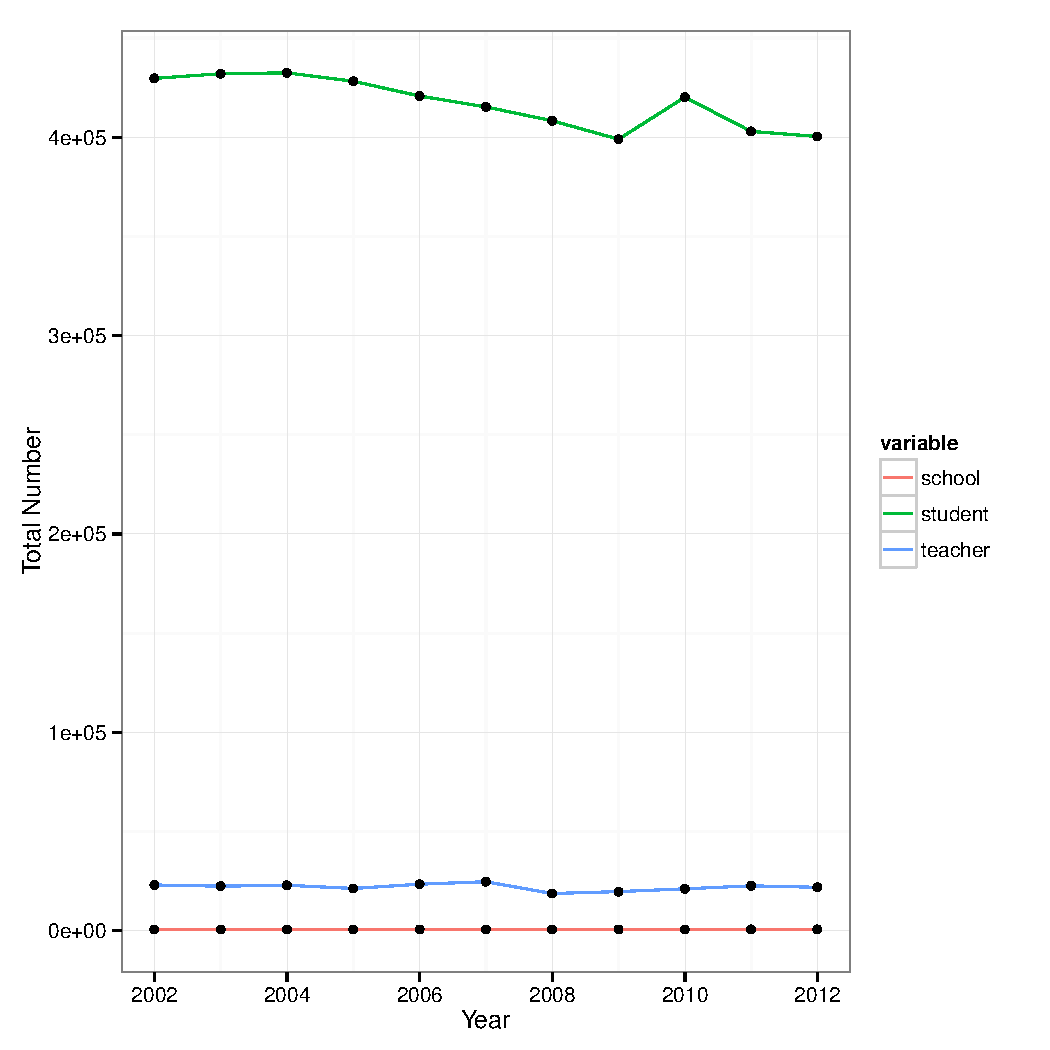
\includegraphics[width=\maxwidth]{figure/chunk8-1} 

\end{knitrout}
\caption{A line graph showing the total schools, students and teachers in Chicago,IL}
  \label{fig:graph}
\end{figure}
Figure~\ref{fig:graph} shows a line graph of total schools, students and teachers
in Chicago, IL\newpage

The graph has three different colored lines. The red, green and blue colored lines are of the school, student and teacher variable, respectively. The X-axis shows the year from December,2001 through December, 2011. The Y-axis shows the total number or count.
\\ The total number of schools in 2001 was 573. It has some rise and fall in the total number. Finally, it became 620 in the year 2011.
\\ The total number of students in 2001 was around 429,684, which decreased to around 399,013 in 2008. It again increased in 2009 to around 420,193 and finally decreased to 400,383 in 2011.
\\ The total number of teachers in 2001 was 23,012, which reached its highest peak of around 24,659 in 2006. Later it decreased to around 18,715 in 2007. It again increased to around 22,589 in 2010 and finally fell to around 21,847 in 2011.
\end{document}
